\chapter{Konzept und Architektur}

In diesem Kapitel wird das konzeptionelle und technische Fundament des entwickelten Systems beschrieben. 
Ziel ist es, eine skalierbare, fehlertolerante und reaktive Architektur zu realisieren, die sowohl Live-Daten 
als auch historische Daten effizient verarbeiten kann. Diese Daten werden in das System integriert, verwaltet 
und so aufbereitet, dass sie für nachgelagerte Komponenten leicht zugänglich und weiterverarbeitbar sind. 
Im weiteren Verlauf werden zunächst die Grundlagen der Skalierbarkeit erläutert, bevor die Systemarchitektur, 
die Rollen der Cluster-Komponenten sowie die Kommunikations- und Datenflüsse innerhalb des Systems vorgestellt 
werden.

\section{Skalierbarkeit und Motivation}

Ein zentraler Aspekt des Projekts ist die effiziente Verarbeitung großer Datenmengen in Echtzeit. 
Im Kontext der Formel-1-Datenanalyse entstehen pro Rennen mehrere hunderttausend Datensätze, 
die eine Vielzahl unterschiedlicher Informationen umfassen, von Telemetriedaten über Zwischenzeiten, 
Positionswechsel und Boxenstopps bis hin zu Sektorzeiten. Diese Datenströme sollen parallel verarbeitet 
und in aggregierter Form zur Darstellung der aktuellen Rennsituation der einzelnen Fahrer bereitgestellt werden.

Um sicherzustellen, dass das System auch bei steigender Datenrate zuverlässig arbeitet, muss es skalierbar ausgelegt sein. 
Skalierbarkeit beschreibt die Fähigkeit eines Softwaresystems, seine Leistungsfähigkeit durch das Hinzufügen von Ressourcen zu erhöhen, 
ohne Änderungen an der Anwendung selbst vornehmen zu müssen \parencite{bass2021}. Ein skalierbares System kann 
somit wachsende Datenmengen oder Benutzeranforderungen verarbeiten, ohne dass ein vollständiges Redesign erforderlich wird.

Im Rahmen dieses Projekts wird eine horizontale Skalierung realisiert. 
Die Anwendung kann als verteiltes System mit mehreren Knoten betrieben werden, 
wobei die einzelnen Rollen des Systems entweder gemeinsam in einem Prozess oder getrennt auf unterschiedliche 
Knoten verteilt ausgeführt werden können. Diese flexible Ausführungsstrategie ermöglicht sowohl den Betrieb 
als monolithische Anwendung als auch eine skalierte Ausführung über mehrere Prozesse oder physische Maschinen. 
Selbst im monolithischen Modus kann das System dynamisch erweitert werden, indem zusätzliche Prozesse 
in den Cluster eingebunden werden. Durch das Hinzufügen weiterer Knoten wird die Arbeitslast automatisch auf 
mehrere Instanzen verteilt, was sowohl die Gesamtleistung als auch die Fehlertoleranz erhöht. 
Fällt ein Knoten aus, übernehmen verbleibende Instanzen mit derselben Rolle automatisch deren Aufgaben.

Durch den Einsatz von Akka.NET und dem Cluster Sharding Mechanismus 
können neue Knoten nach ihrer Registrierung am Hauptknoten dynamisch in das System integriert werden. 
Nach dem Beitritt zum Cluster übernehmen sie automatisch Teile der Verarbeitung, 
ohne dass Konfigurationsänderungen oder Neustarts erforderlich sind.
Dieses Skalierungsprinzip führt zu einer flexiblen und anpassungsfähigen Architektur,
bei der neu hinzukommende Prozesse automatisch in den Cluster integriert werden,
ohne dass zusätzliche Konfigurationsschritte erforderlich sind.

\section{Gesamtarchitektur des Systems}
Die Architektur des entwickelten Systems basiert auf dem Akka.NET-Framework und nutzt dessen 
Cluster-Mechanismen zur Realisierung einer verteilten, fehlertoleranten und skalierbaren Anwendung.
Abbildung \ref{fig:own-architecture} zeigt die zentralen Komponenten des Systems und deren Interaktion.

\begin{figure}[H]
    \centering
    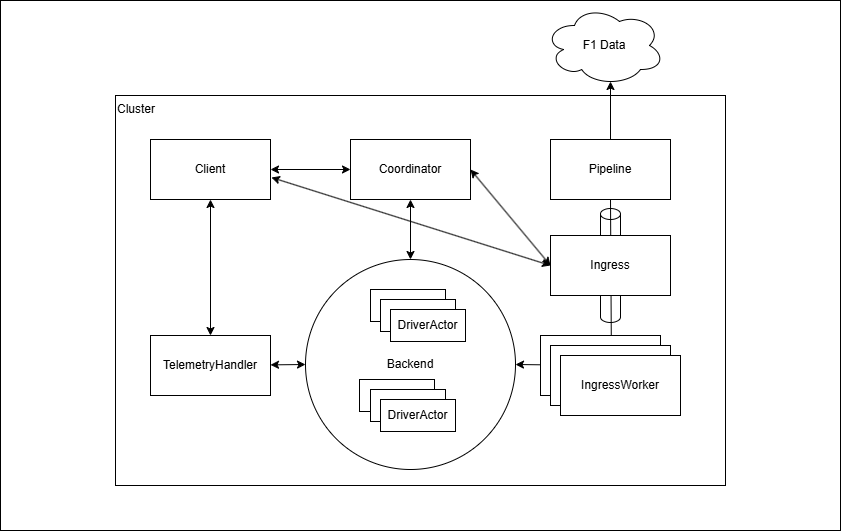
\includegraphics[width=0.8\textwidth]{assets/architecture.v1.png}
    \caption{Architekturübersicht des Projekts}
    \label{fig:own-architecture}
\end{figure}

Das System besteht aus mehreren Knoten, die unterschiedliche Rollen übernehmen. Für den Betrieb 
des Clusters sind grundsätzlich zwei Ausführungsmodi vorgesehen:

\begin{itemize}
    \item \textbf{Monolithischer Modus:} 
    In diesem Modus werden alle Rollen innerhalb eines einzelnen Prozesses ausgeführt.
    Diese Variante eignet sich insbesondere für Entwicklungs- und Testzwecke, da sie die Systemkomplexität 
    reduziert und die Einrichtung vereinfacht.
    \item \textbf{Verteilte Ausführung:} 
    Hierbei werden die verschiedenen Rollen auf separate Prozesse oder physische Maschinen verteilt.  
    Dadurch wird eine effizientere Ressourcennutzung ermöglicht und das System kann bei steigender Last 
    horizontal skaliert werden, da einzelne Komponenten unabhängig voneinander erweitert werden können.
\end{itemize}

Jeder Knoten im Cluster kann eine der folgenden Rollen übernehmen: Ingress, Backend und Coordinator.
Diese Rollen sind für die verschiedenen Aufgaben innerhalb des Systems verantwortlich und arbeiten zusammen, 
um die Verarbeitung und Bereitstellung der Daten sicherzustellen.

Zur Verwaltung und strukturierten Weiterleitung der Daten wird das Cluster-Sharding-Konzept von Akka.NET eingesetzt.
Damit Nachrichten effizient an die jeweilige ShardRegion gesendet und von dieser empfangen werden können, 
kommen Proxies zum Einsatz, die als Vermittler zwischen den Knoten und den Shards fungieren.

Ein integrierter Load Balancer verteilt eingehende Datenströme aus externen Quellen gleichmäßig 
auf mehrere Arbeitsknoten.Diese Knoten leiten die empfangenen Daten anschließend an die zuständige 
ShardRegion weiter, wo sie verarbeitet und persistiert werden.

Um die Kommunikation zwischen den verteilten Komponenten sicherzustellen, wird zudem ein verteiltes 
Publish/Subscribe-System eingesetzt.Dieses ermöglicht es den verschiedenen Rollen, Nachrichten 
asynchron auszutauschen und auf Ereignisse zu reagieren, ohne dass direkte Verbindungen erforderlich sind.


\section{Rollen im Cluster}

Dieses Kapitel beschreibt die drei Hauptrollen innerhalb des Clusters: Ingress, Backend 
und Coordinator. Jede dieser Rollen erfüllt eine klar abgegrenzte Funktionalität und trägt 
gemeinsam zur Gesamtfunktionalität des Systems bei.

\subsection{Ingress}

Der Ingress-Knoten ist für die Datenbeschaffung und -weiterleitung an die ShardRegion zuständig.
Die Kommunikation erfolgt über Proxies, die als Vermittler zwischen den eingehenden Datenströmen 
und den zuständigen Shards fungieren.

Zur Steuerung des Datenflusses wird Akka.Streams verwendet, wodurch eingehende Datenströme 
effizient verarbeitet werden können. Bei hohen Datenmengen sorgen integrierte Backpressure-Mechanismen 
dafür, dass keine Überlastung der Arbeitsknoten entsteht. Um Datenverluste zu vermeiden, sendet 
der Ingress-Knoten neue Daten erst dann an die Arbeitsknoten weiter, wenn eine Bestätigung der 
ShardRegion vorliegt. Dies gewährleistet eine kontrollierte und zuverlässige Datenaufnahme 
innerhalb des Clusters.

\subsection{Backend}

Der Backend-Knoten ist für die eigentliche Verarbeitung und Speicherung der eingehenden Daten 
verantwortlich. Er empfängt die Daten vom Ingress-Knoten und speichert sie in einer Datenstruktur, 
die als Modell für die Formel-1-Daten dient. Nach erfolgreicher Verarbeitung und Speicherung werden 
die aufbereiteten Daten über einen sogenannten Händler-Knoten an die entsprechenden Konsumenten 
weitergeleitet.

Zur Sicherstellung der Datenpersistenz werden die Informationen entweder in einer In-Memory-Datenbank 
oder einer PostgreSQL-Datenbank abgelegt.Um Datenverluste bei Ausfällen oder Neuzuweisungen von 
Backends zu verhindern, kommt die Akka.Persistence-Funktionalität zum Einsatz. Dabei werden regelmäßig 
sogenannte Snapshots erstellt, anstatt jede einzelne Änderung sofort zu 
speichern.
Dies reduziert die Datenbanklast und gewährleistet gleichzeitig eine schnelle Wiederherstellung.

Nach einem Neustart oder einem Failover kann der aktuelle Zustand durch das Wiederherstellen der 
gespeicherten Snapshots und das erneute Abspielen der nachfolgenden Events rekonstruiert werden.

\subsection{Coordinator}

Der Coordinator-Knoten übernimmt die Verwaltung und Überwachung des Clusters.Er stellt sicher, 
dass die verschiedenen Komponenten reibungslos zusammenarbeiten und auf neu beitretende oder 
ausgefallene Knoten korrekt reagieren.

Eine zentrale Aufgabe des Coordinators besteht darin, den Zustand der ShardRegion zu überwachen.
Falls keine funktionsfähige Region verfügbar ist, beispielsweise nach einem Node-Ausfall oder 
während einer Rebalancing-Phase, verhindert der Coordinator, dass der Ingress-Knoten weiterhin 
Daten an die ShardRegion sendet. Er fungiert somit als Kontrollinstanz, die sicherstellt, 
dass Daten nur dann in den Cluster eingespeist werden, wenn eine stabile und empfangsbereite 
Verarbeitungseinheit vorhanden ist.

Darüber hinaus übernimmt der Coordinator allgemeine Verwaltungs- und Überwachungsaufgaben, 
wie das Erfassen von Clusterstatusmeldungen oder das Weiterleiten relevanter Ereignisse an 
andere Komponenten.

\section{Cluster Sharding}

Cluster Sharding ist ein Mechanismus, der es Cluster-Akteuren ermöglicht, über ihre logischen IDs 
zu kommunizieren, ohne die physischen Standorte der Zielakteure kennen zu müssen \parencite{getakka_cluster_sharding}.  
Es handelt sich um ein Werkzeug, das die verteilte Verwaltung zustandsbehafteter Akteure über 
mehrere Knoten innerhalb eines Clusters ermöglicht \parencite{cluster_sharding_petabridge}.  

Der strukturelle Aufbau des Cluster Shardings ist wie folgt gegliedert:

\begin{figure}[H]
    \centering
    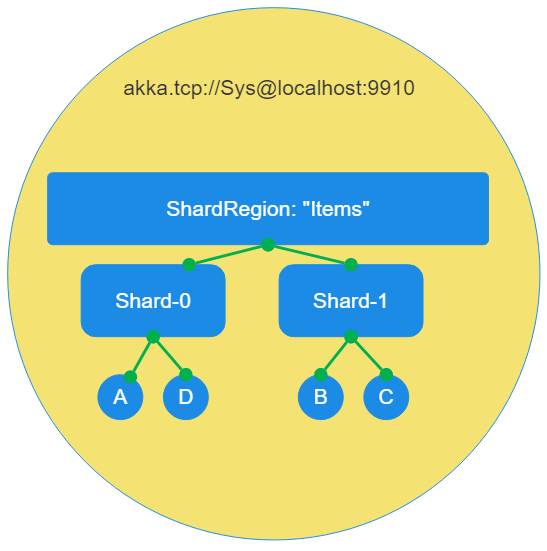
\includegraphics[width=0.5\textwidth]{assets/cluster-sharding.png}
    \caption{Cluster Sharding Architektur \parencite{cluster_sharding_petabridge}}
    \label{fig:architecture}
\end{figure}

\begin{itemize}
    \item \textbf{ShardRegion:}
    Die ShardRegion ist eine Instanz, die als zentraler Einstiegspunkt für alle Nachrichten an die im 
    Cluster verteilten Entitäten dient. Sie übernimmt das Routing eingehender Nachrichten, indem sie 
    anhand der Entity-ID ermittelt, welche Shard und welcher Knoten für die Verarbeitung zuständig ist.
    Neben der reinen Nachrichtenverteilung steuert die ShardRegion auch den Lebenszyklus der Entitäten. 
    Sie erstellt Entitäten bei Bedarf, kann sie passivieren, wenn sie längere Zeit nicht genutzt werden, 
    und organisiert ihre Neuzuweisung im Falle von Clusteränderungen.
    \parencite{cluster_sharding_petabridge}

    \item \textbf{Shard:}
    Die Shard stellt die eigentliche Verteilungseinheit im Cluster dar. Sie definiert, auf welchem Knoten 
    sich eine Gruppe von Entitäten befindet und übernimmt die Verwaltung dieser Entitäten. Intern agiert 
    sie als übergeordneter Akteur und organisiert jede Entität gemäß dem Child-per-Entity-Muster.
    \parencite{cluster_sharding_petabridge}

    \item \textbf{Entity:}
    Die Entität ist die kleinste Verarbeitungseinheit im Cluster Sharding. Sie repräsentiert einen konkreten, 
    zustandsbehafteten Akteur, der über eine eindeutige ID identifiziert wird und Nachrichten eigenständig 
    empfangen und verarbeiten kann.
    \parencite{cluster_sharding_petabridge}
\end{itemize}

Das Ziel des Cluster Shardings besteht darin, sicherzustellen, dass im gesamten Cluster stets genau eine Instanz 
jeder Entität existiert. Darüber hinaus wird eine gleichmäßige Verteilung der Entitäten über alle verfügbaren 
Knoten angestrebt, um eine optimale Ressourcenauslastung und Lastverteilung zu gewährleisten. Dies wird durch den 
Einsatz von Hashing-Algorithmen erreicht, die bestimmen, auf welchem Knoten eine bestimmte Entität platziert wird.

Die ShardRegion ist zudem für das Rebalancing verantwortlich, also die Umverteilung von Shards, wenn Knoten dem 
Cluster beitreten oder diesen verlassen. Sie koordiniert außerdem den gesamten Lebenszyklus der Entitäten, 
indem sie diese bei Bedarf erstellt, passiviert oder entfernt.
\parencite{cluster_sharding_petabridge}

\subsection{Neuausgleich der Shards}

Ein zentraler Aspekt des Cluster Shardings ist der Neuausgleich (Rebalancing) der Shards. Dieser Prozess wird vom 
Shard-Koordinator gesteuert, der alle beteiligten Akteure im Cluster darüber informiert, dass die Übergabe einer 
Shard begonnen hat. Während der Migration werden eingehende Nachrichten für die betroffene Shard zunächst 
zwischengespeichert. Sobald die Übertragung abgeschlossen ist, werden die bisherigen Shard-Instanzen beendet und 
die gespeicherten Nachrichten an die neuen Shard-Instanzen weitergeleitet.

Während dieses Vorgangs wird der Zustand der Entitäten nicht automatisch migriert. Um Datenverlust zu vermeiden, 
sollten Entitäten daher so implementiert sein, dass ihr Zustand persistent gespeichert und bei Bedarf 
wiederhergestellt werden kann.
\parencite{cluster_sharding_petabridge}

Die Logik des Rebalancing kann bei Bedarf durch eine benutzerdefinierte Zuweisungsstrategie angepasst werden. 
Standardmäßig verwendet Akka.NET eine Hash-basierte Verteilung, um eine gleichmäßige Auslastung der verfügbaren 
Knoten sicherzustellen.
\parencite{getakka_cluster_sharding}

\subsection{ShardRegion-Proxy}

Ein ShardRegion-Proxy wird benötigt, wenn eine Kommunikation mit einer ShardRegion stattfindet, die sich nicht 
auf demselben Knoten befindet.
\parencite{getakka_cluster_sharding}

In diesem System liegt die ShardRegion ausschließlich auf Knoten mit der Rolle \textit{Backend}. Daher muss ein 
Proxy verwendet werden, wenn Komponenten außerhalb dieser Rolle Nachrichten an die ShardRegion senden sollen.

\section{Singleton}

Der Cluster-Singleton gewährleistet, dass eine bestimmte Aktor-Instanz innerhalb des gesamten Clusters exakt einmal 
existiert. Dieses Konzept wird eingesetzt, wenn Aufgaben zentral ausgeführt werden müssen und eine Mehrfachausführung 
zu Inkonsistenzen oder erhöhtem Synchronisationsaufwand führen würde. Typische Einsatzbereiche umfassen globale 
Verwaltungsfunktionen, zentrale Namensauflösung oder Routinglogik.

Ein Vorteil dieser Architektur ist, dass wichtige Entscheidungen und Aufgaben an einer Stelle gebündelt werden. 
Dadurch entsteht keine Verwirrung darüber, welcher Aktor zuständig ist. Der Nachteil liegt jedoch darin, dass der 
Singleton ein einzelner Engpass sein kann. Wenn er ausfällt oder überlastet wird, kann das Auswirkungen auf das 
gesamte System haben.

Die Bereitstellung der Singleton-Instanz erfolgt auf Knoten, die über eine vordefinierte Rolle verfügen. Existieren 
mehrere Knoten mit dieser Rolle, wird die Instanz üblicherweise auf dem Knoten mit der längsten Cluster-Mitgliedschaft 
ausgeführt. Im Falle eines Ausfalls übernimmt automatisch ein anderer geeigneter Knoten die Ausführung des Singletons, 
wodurch eine hohe Verfügbarkeit gewährleistet bleibt.
\parencite{getakka_singleton}

\subsection{Singleton-Proxy}

Um auf den Cluster-Singleton zugreifen zu können, wird ein Singleton-Proxy verwendet. Dieser ermöglicht es allen 
Komponenten innerhalb des Clusters, Nachrichten an den Singleton zu senden, ohne dessen tatsächlichen Ausführungsort 
kennen zu müssen. Die Identifikation erfolgt über einen definierten Marker, sodass keine explizite Actor- oder 
Netzwerkadresse notwendig ist.

Falls der Singleton vorübergehend nicht erreichbar ist, werden eingehende Nachrichten im Proxy gepuffert und nach 
Wiederherstellung der Verbindung automatisch weitergeleitet. Wird die maximale Puffergöße überschritten, verwirft 
der Proxy die ältesten Nachrichten, um eine Überlastung zu verhindern.
\parencite{getakka_singleton}

\section{Kommunikation über Verteiltes Pub/Sub}

Der Einsatz verteilter Kommunikation in Akka.NET erfolgt immer dann, wenn Nachrichten nicht mehr nur innerhalb 
eines einzelnen Aktorensystems ausgetauscht werden, sondern zwischen mehreren Systemen verteilt kommuniziert wird, 
unabhängig davon auf welchen physischen oder virtuellen Maschinen diese Systeme betrieben werden. In Abbildung 
\ref{fig:distribute-pub-sub} ist eine solche verteilte Publish Subscribe Architektur veranschaulicht.

\begin{figure}[H]
    \centering
    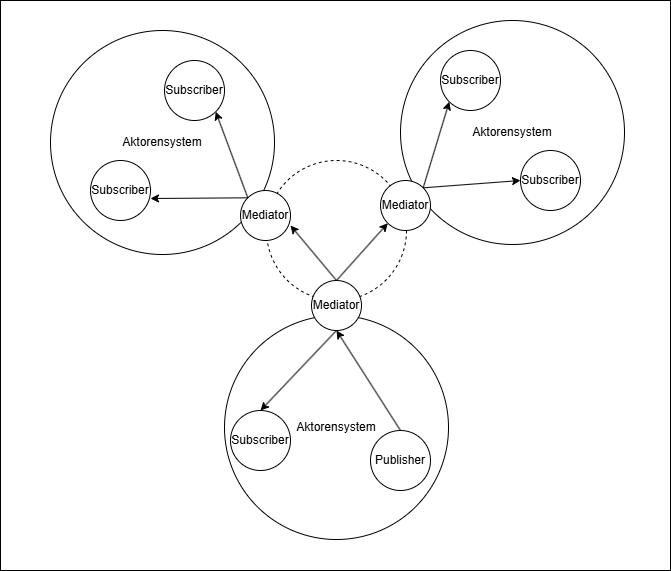
\includegraphics[width=0.7\textwidth]{assets/dis-p_s.png}
    \caption{Verteiltes Publish-Subscribe Architektur \parencite{distributed_petabridge}}
    \label{fig:distribute-pub-sub}
\end{figure}

Für die Kommunikation registriert sich ein Aktor, der Ereignisse von anderen Aktoren empfangen möchte, bei seinem 
lokalen Mediator unter Angabe eines Topics oder eines Aktorenpfads. Nach der Registrierung erhält der abonnierende 
Aktor eine Bestätigungsmeldung womit sichergestellt wird, dass er nun Nachrichten über das entsprechende Topic 
empfangen kann.

Wenn ein Aktor eine Nachricht an alle Abonnenten eines Topics senden möchte, informiert er ebenfalls seinen lokalen 
Mediator durch eine Publikationsnachricht und gibt dabei das betreffende Topic oder den Zielpfad an. In Szenarien, 
in denen eine Nachricht nur an einen einzelnen Abonnenten gesendet werden soll, ist dies ebenfalls möglich. 
Standardmäßig erfolgt die Zustellung dabei zufällig an einen der Teilnehmer der Abonnentengruppe.
\parencite{distributed_petabridge}

\section{Streams}



\subsection{Overflowstrategien}


\section{Alternative Architekturvarianten}
